\documentclass[aspectratio=169]{beamer}
\usepackage{babel}
% \usepackage[german]{babel}

\usepackage{tikz, transparent, colortbl, listings, pgfplots}
\usepackage[export]{adjustbox}
\usepackage[skins,theorems]{tcolorbox}
 
\usetikzlibrary{automata,positioning}
\setbeamercovered{transparent}
\pgfplotsset{compat=1.18}
\tcbset{highlight math style={enhanced,colframe=red,colback=white,arc=0pt,boxrule=1pt}}

%
% Cited from Ausarbeitung/aspdoc.cls
%
\lstset{
    language=C++,
    basicstyle=\upshape\footnotesize\ttfamily,
    numbers=left,                   % where to put the line-numbers
    numberstyle=\tiny\color{gray},  % the style that is used for the line-numbers
    numbersep=5pt,                  % how far the line-numbers are from the code
    showstringspaces=false,
    frame=single,                   % adds a frame around the code
    rulecolor=\color{black},
    tabsize=2,                      % sets default tabsize to 2 spaces
    captionpos=b,                   % sets the caption-position to bottom
    breaklines=true,                % sets automatic line breaking
    breakatwhitespace=false,        % sets if automatic breaks should only happen at whitespace
    title=\lstname,                 % show the filename of files included with \lstinputlisting;
    keywordstyle=\color{blue},      % keyword style
    commentstyle=\color{dkgreen},   % comment style
    stringstyle=\color{mauve},      % string literal style
    escapeinside={\%*}{*)},         % if you want to add LaTeX within your code
}

% Useful Read:
% https://www.overleaf.com/learn/latex/Beamer

\title{Molecular Dynamics}
\subtitle{Group A}
\author{Haoyuan Ma \and Zhengying Zhao \and Anatoly Weinstein}
\date{31st of October 2025}

\newcommand{\framebackground}[2]{
    \begin{tikzpicture}
        \transparent{#1}
        \node[inner sep=0] at (current page.center) {
            
\includegraphics[height=\paperheight, right]{./media/tum-uhrenturm.png}
        };
        \transparent{1}
        \node[anchor=south, text width=\paperwidth, text height=1.5cm, draw=none, align=center] at (current page.south) {
            \insertpagenumber
        };
        \transparent{#2}
        \node[anchor=south, text width=\paperwidth, text height=1.5cm, draw=none, align=right] at (current page.south) {
            \small Haoyuan Ma, Zhengying Z, Anatoly W. \,\,
        };
    \end{tikzpicture}
}

\newcommand{\headerframe}{
    \usebackgroundtemplate{
        \framebackground{0.2}{1}
    }
}

\newcommand{\simpleframe}{
    \usebackgroundtemplate{
        \framebackground{0}{1}
    }
}

\newcommand{\blue}[1]{{\color{beamer@blendedblue} #1}}
\newcommand{\yellow}[1]{{\color[HTML]{AF8F10} #1}}
\newcommand{\gray}[1]{{\color[HTML]{8F8F8F} #1}}
\newcommand{\red}[1]{{\color[HTML]{FF5F5F} #1}}

\begin{document}

%
% Frame
%
\usebackgroundtemplate{\framebackground{0.2}{0}}
\begin{frame}
    \maketitle
\end{frame}

\simpleframe\begin{frame}{The test run of the simulation}
    \begin{figure}
        \centering
        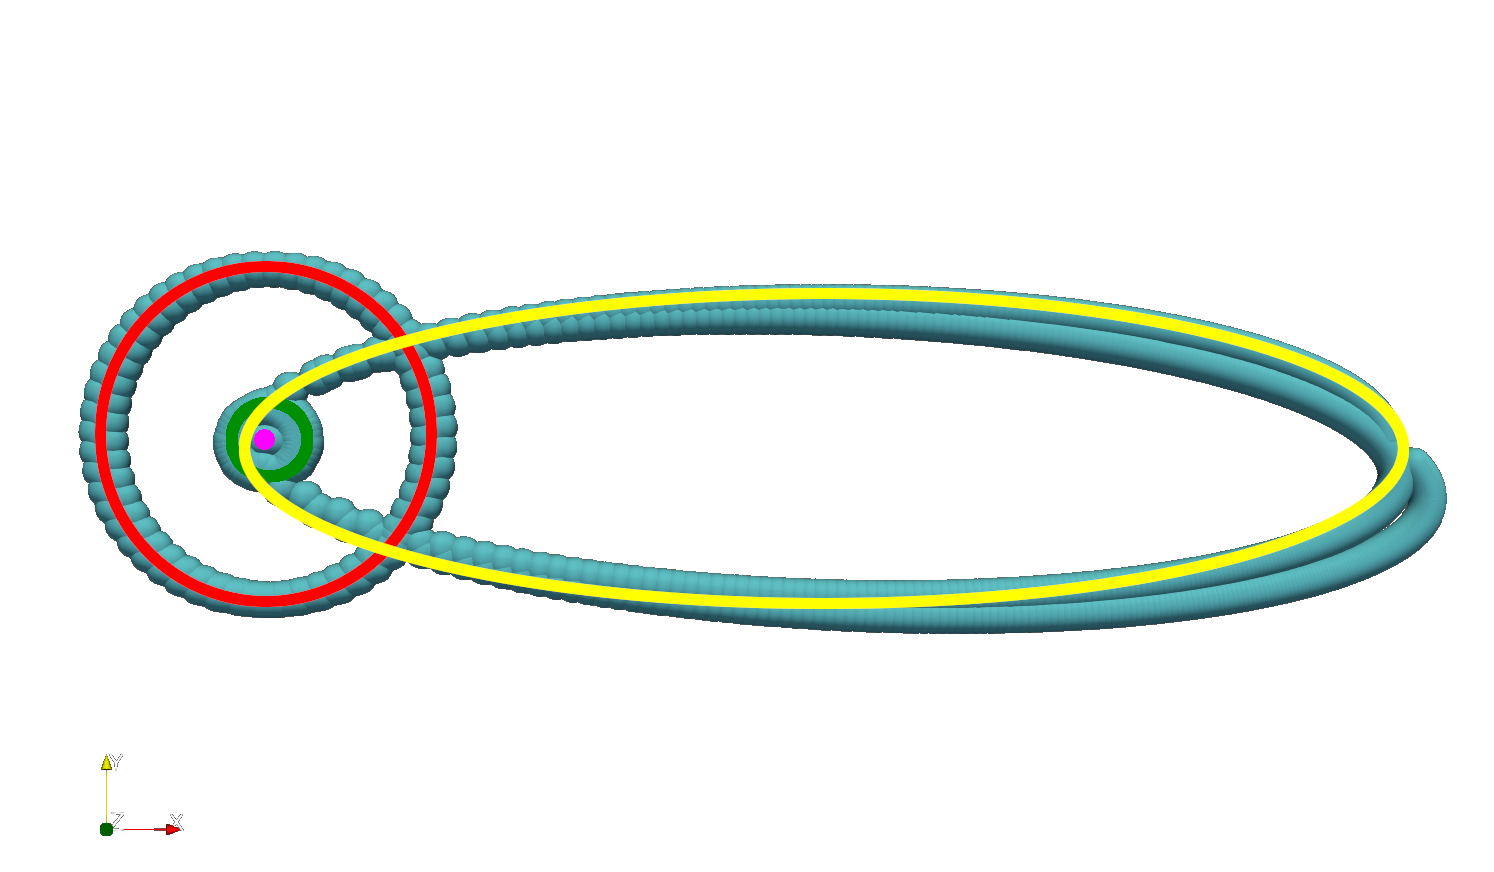
\includegraphics[width=0.7\textwidth]{media/t1000_d0.14_annotated.png}

        \par\vspace{4pt}
        \begin{center}
            {\color[HTML]{FF00FF}$\bullet$}~Sun \qquad
            {\color[HTML]{008F00}$\bullet$}~Earth \qquad
            {\color[HTML]{FF0000}$\bullet$}~Jupiter \qquad
            {\color[HTML]{8F8F00}$\bullet$}~Halley's Comet
        \end{center}
    \end{figure}
\end{frame}

\simpleframe\begin{frame}{The test run of the simulation}
    \begin{figure}
        \centering
        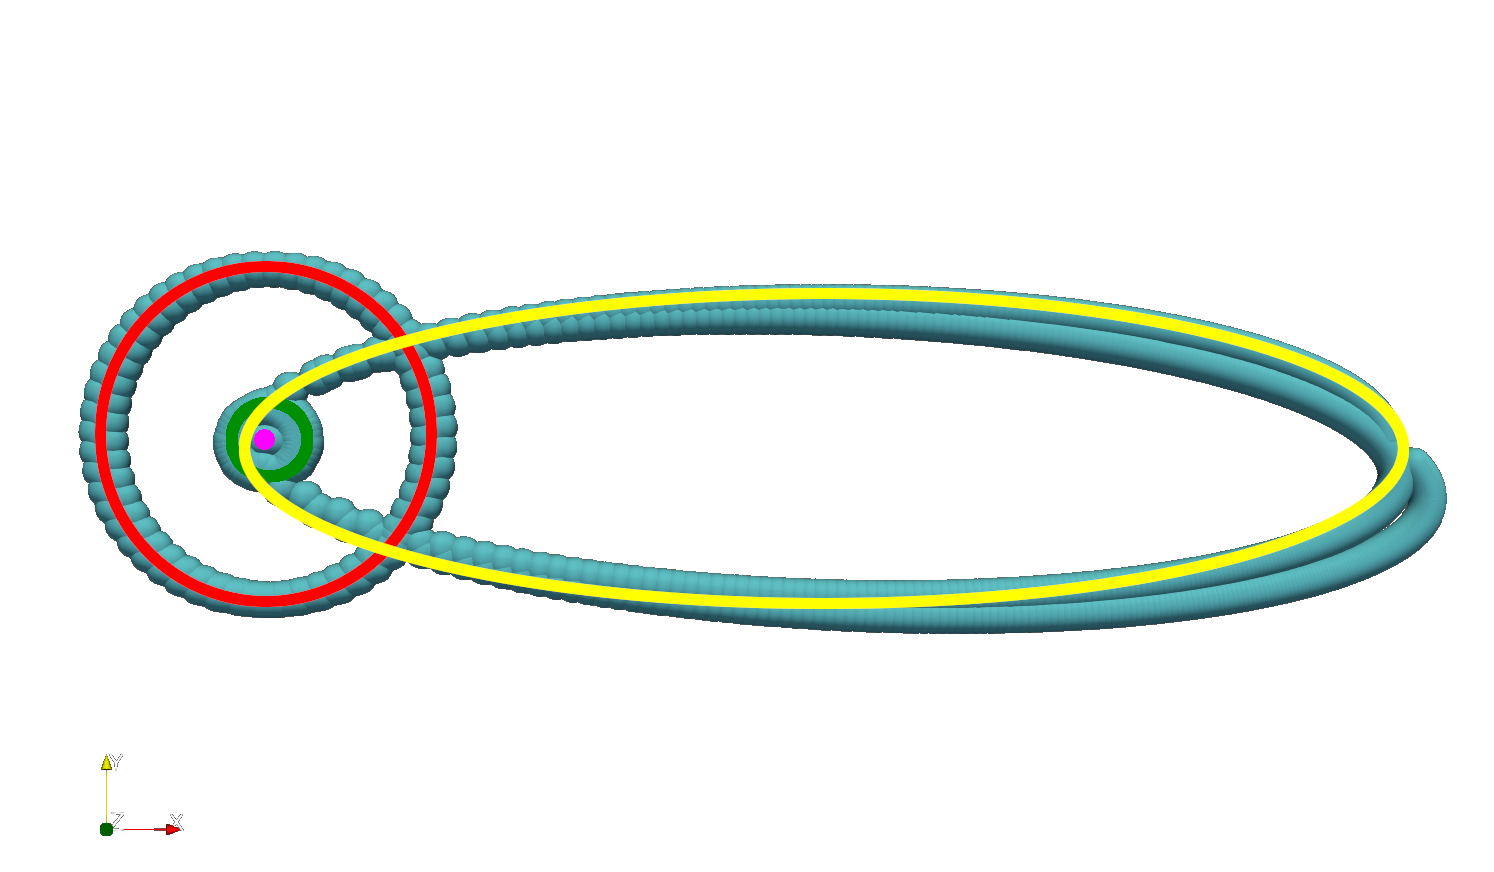
\includegraphics[width=0.5\textwidth]{media/t1000_d0.14_annotated.png}

        \par\vspace{4pt}
        \begin{center}
            {\color[HTML]{FF00FF}$\bullet$}~Sun \gray{($\text{m} = 10^{30} \text{kg}$)} \,
            {\color[HTML]{008F00}$\bullet$}~Earth \gray{($\text{m} = 5.9 \times 10^{24} \text{kg}$)} \,
            {\color[HTML]{FF0000}$\bullet$}~Jupiter \gray{($\text{m} = 10^{27} \text{kg}$)} \,
            % {\color[HTML]{8F8F00}$\bullet$}~Halley's Comet
        \end{center}
    \end{figure}

    Reasoning: $\text{m}_\text{sun} = 1047 \, \text{m}_\text{jupiter}$ and $\text{m}_\text{sun} = 333\,000 \, \text{m}_\text{earth}$ matches input mass relatively.
\end{frame}

\simpleframe\begin{frame}{Comparing $\Delta t$ in Simulations}
    \begin{columns}
        \begin{column}{0.5\textwidth}
            \begin{figure}
                \centering
                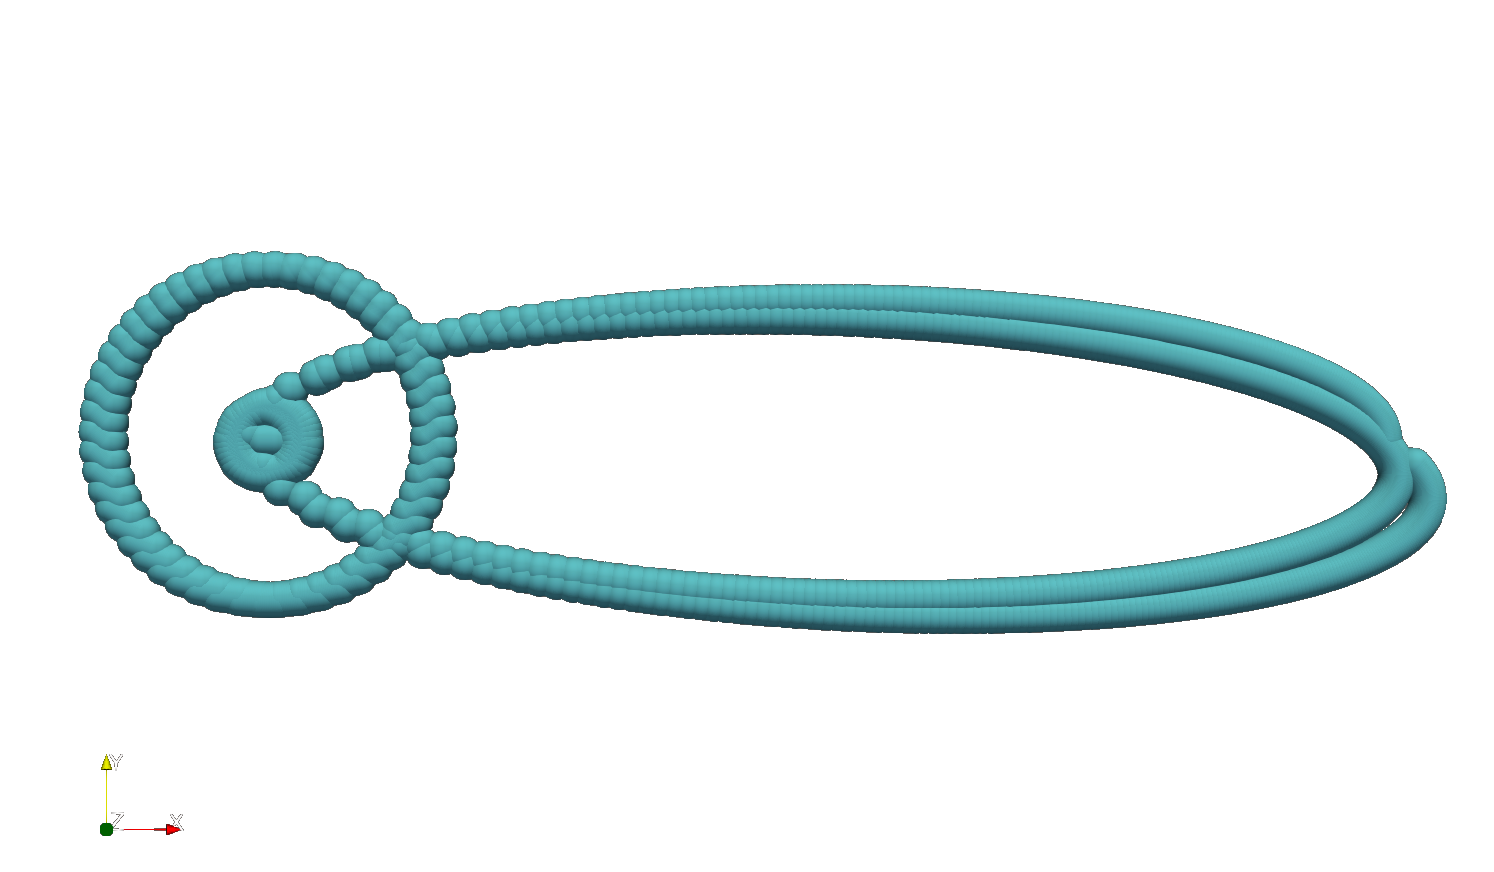
\includegraphics[width=0.6\textwidth]{media/t1000_d0.14.png}
                \caption{Simulation with $\Delta t = 0.14$}
            \end{figure}
        \end{column}
        \begin{column}{0.5\textwidth}
            \begin{figure}
                \centering
                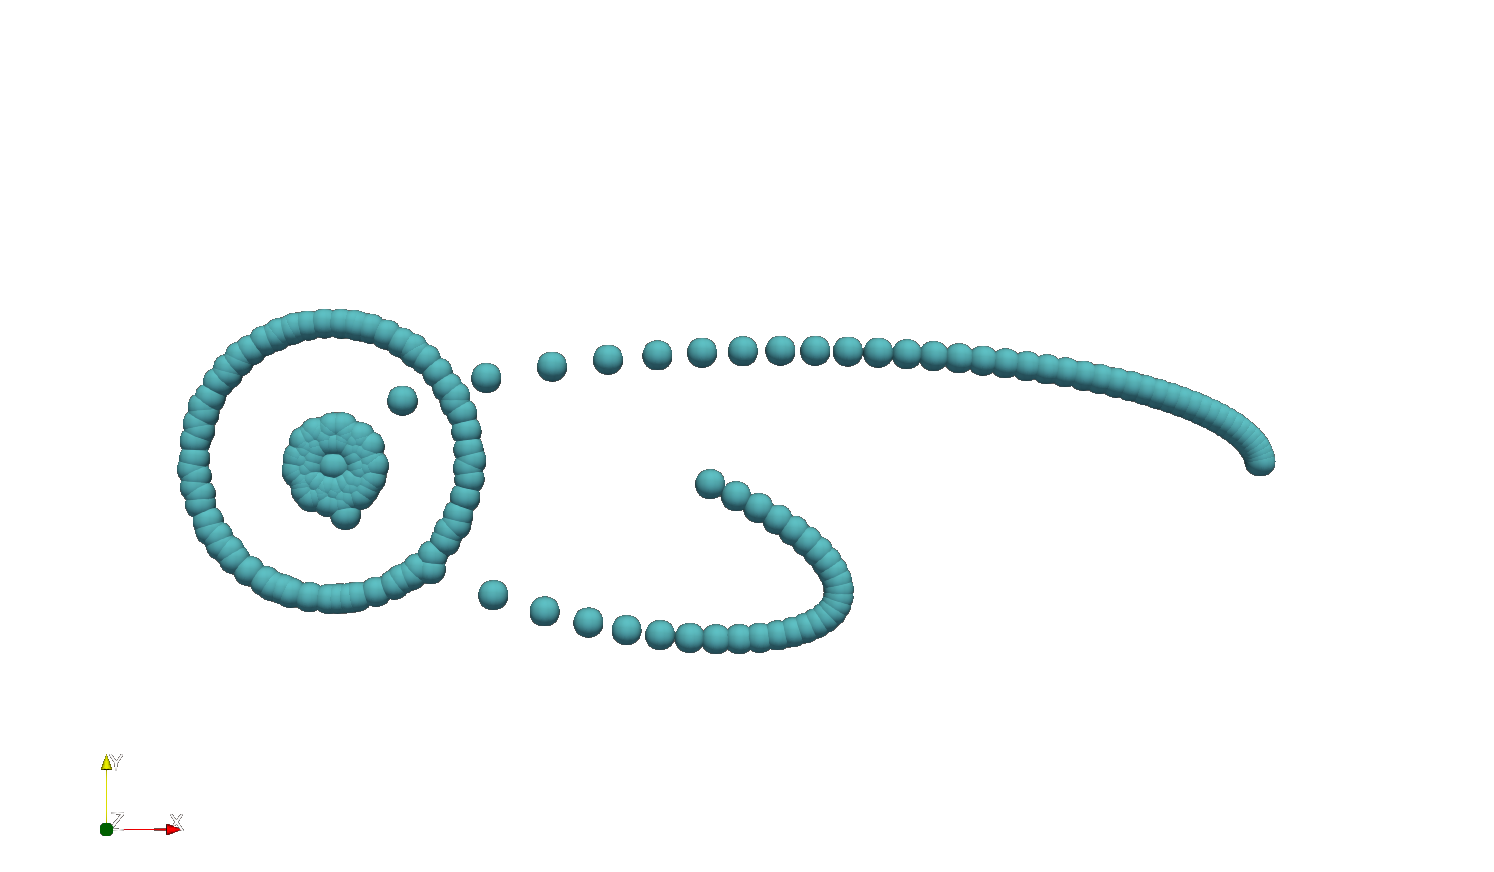
\includegraphics[width=0.6\textwidth]{media/t400_d0.56.png}
                \caption{Simulation with $\Delta t = 0.56$}
            \end{figure}
        \end{column}
    \end{columns}
    
    \begin{figure}
        \centering
        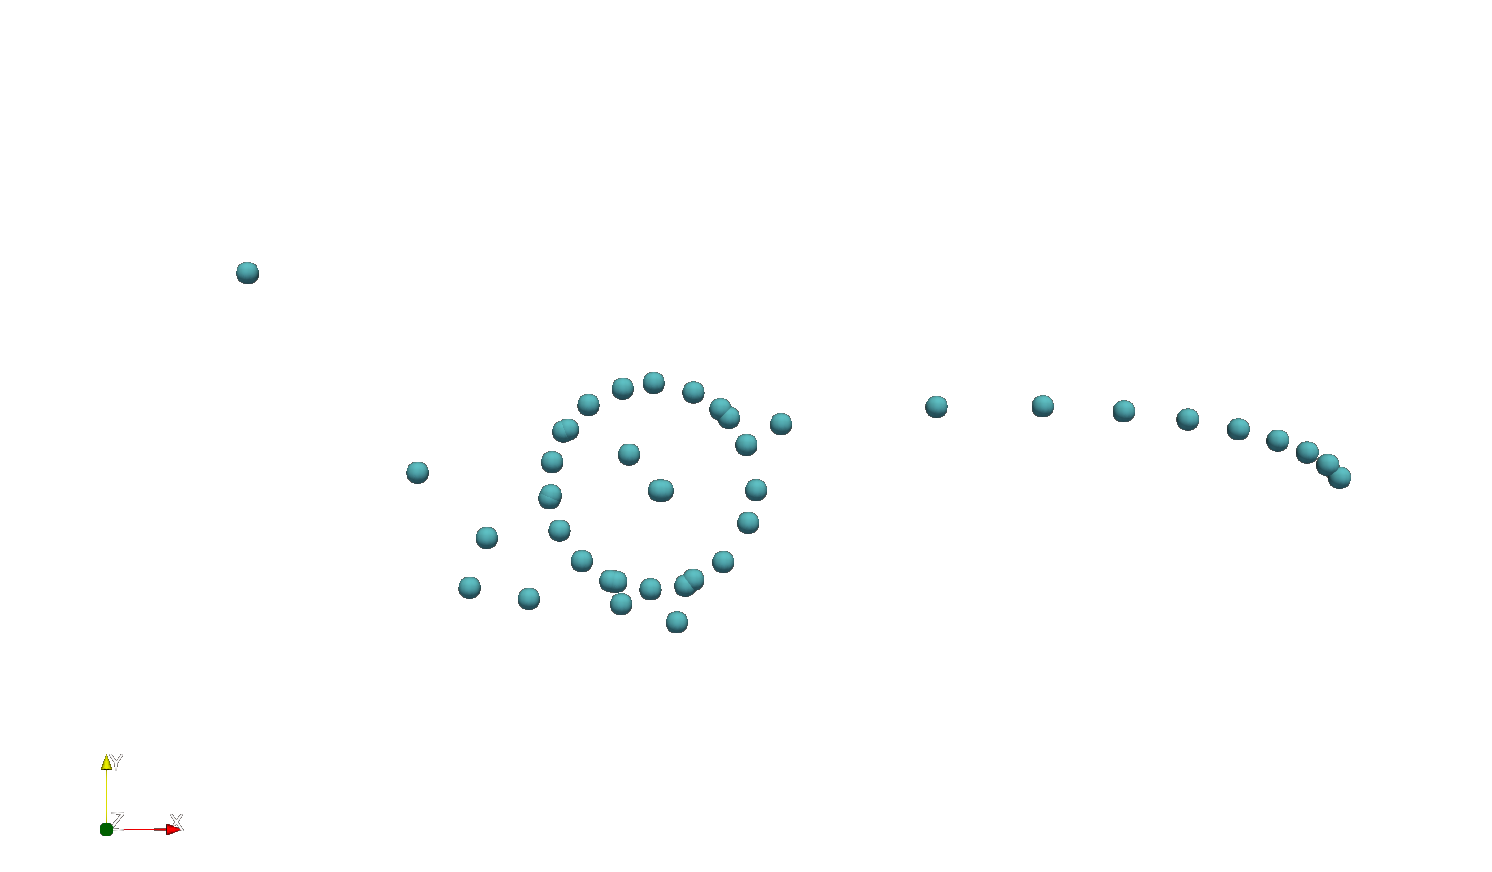
\includegraphics[width=0.3\textwidth]{media/t500_d2.24.png}
        \caption{Simulation with $\Delta t = 2.24$}
    \end{figure}

    \vspace{0.5cm}

    Conclusion: \red{Results deviate for different $\Delta t$!}

    Leads to the question: \blue{How to choose an appropriate $\Delta t$?}
\end{frame}

\simpleframe\begin{frame}{Comparing $\Delta t$ in Simulations}
    \begin{columns}
        \begin{column}{0.3\textwidth}
            \centering
            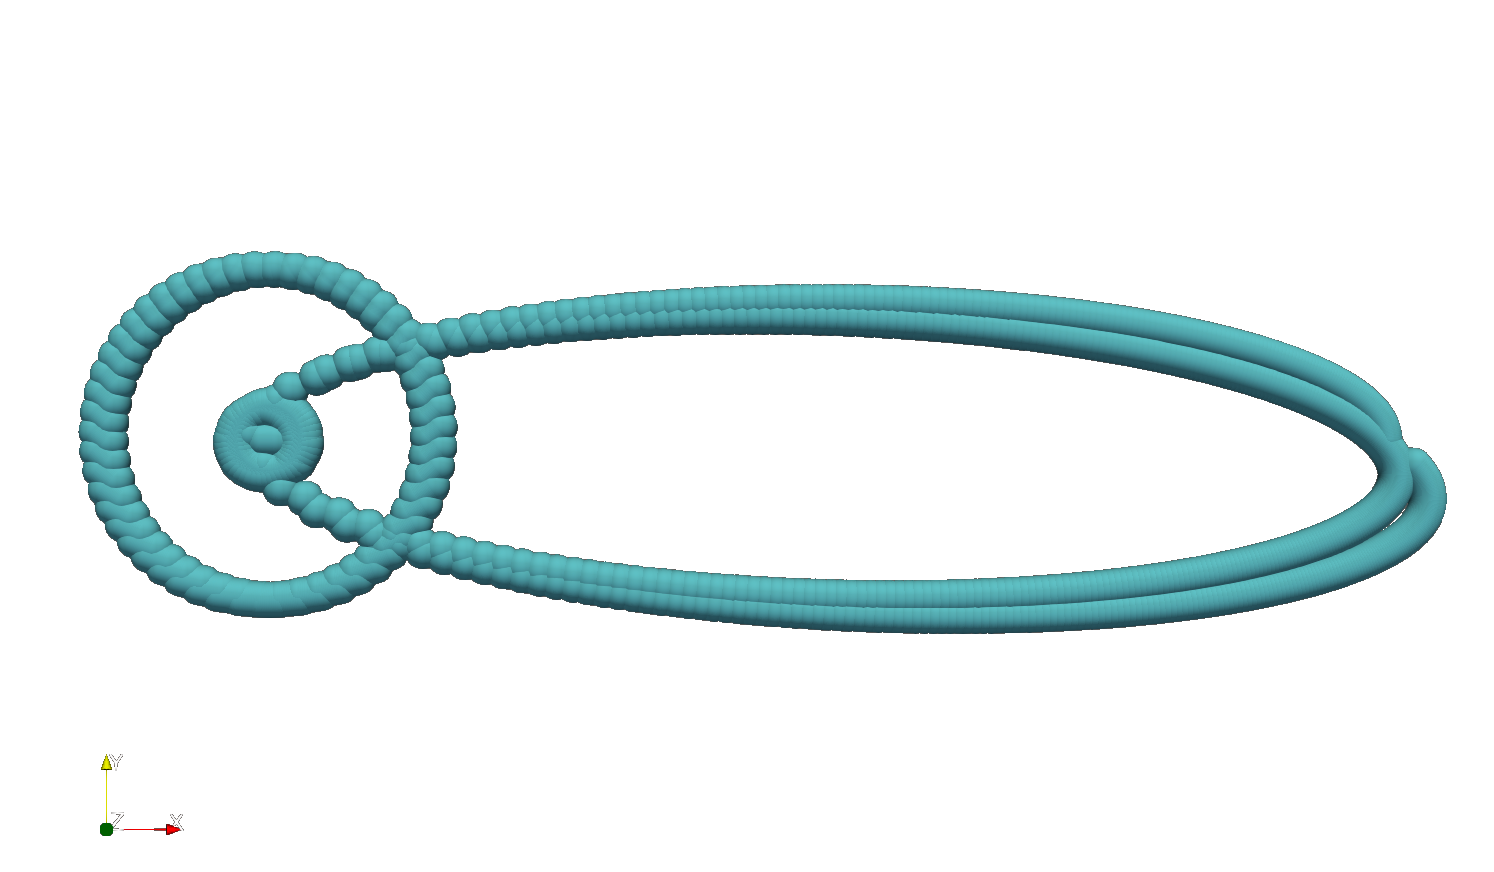
\includegraphics[width=0.9\textwidth]{media/t1000_d0.14.png}
        \end{column}
        \begin{column}{0.3\textwidth}
            \centering
            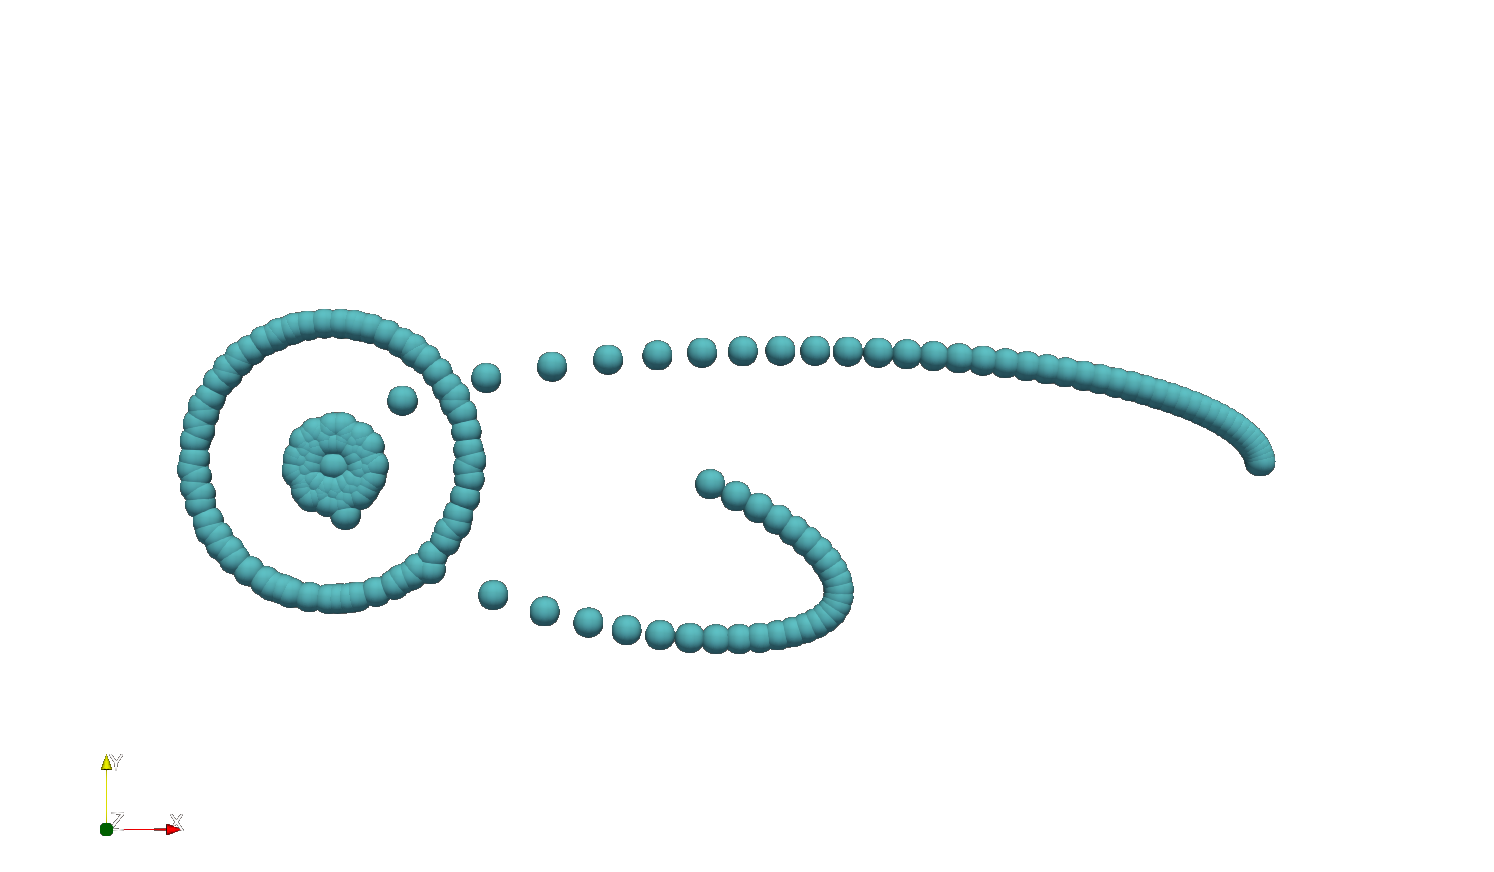
\includegraphics[width=0.9\textwidth]{media/t400_d0.56.png}
        \end{column}
        \begin{column}{0.3\textwidth}
            \centering
            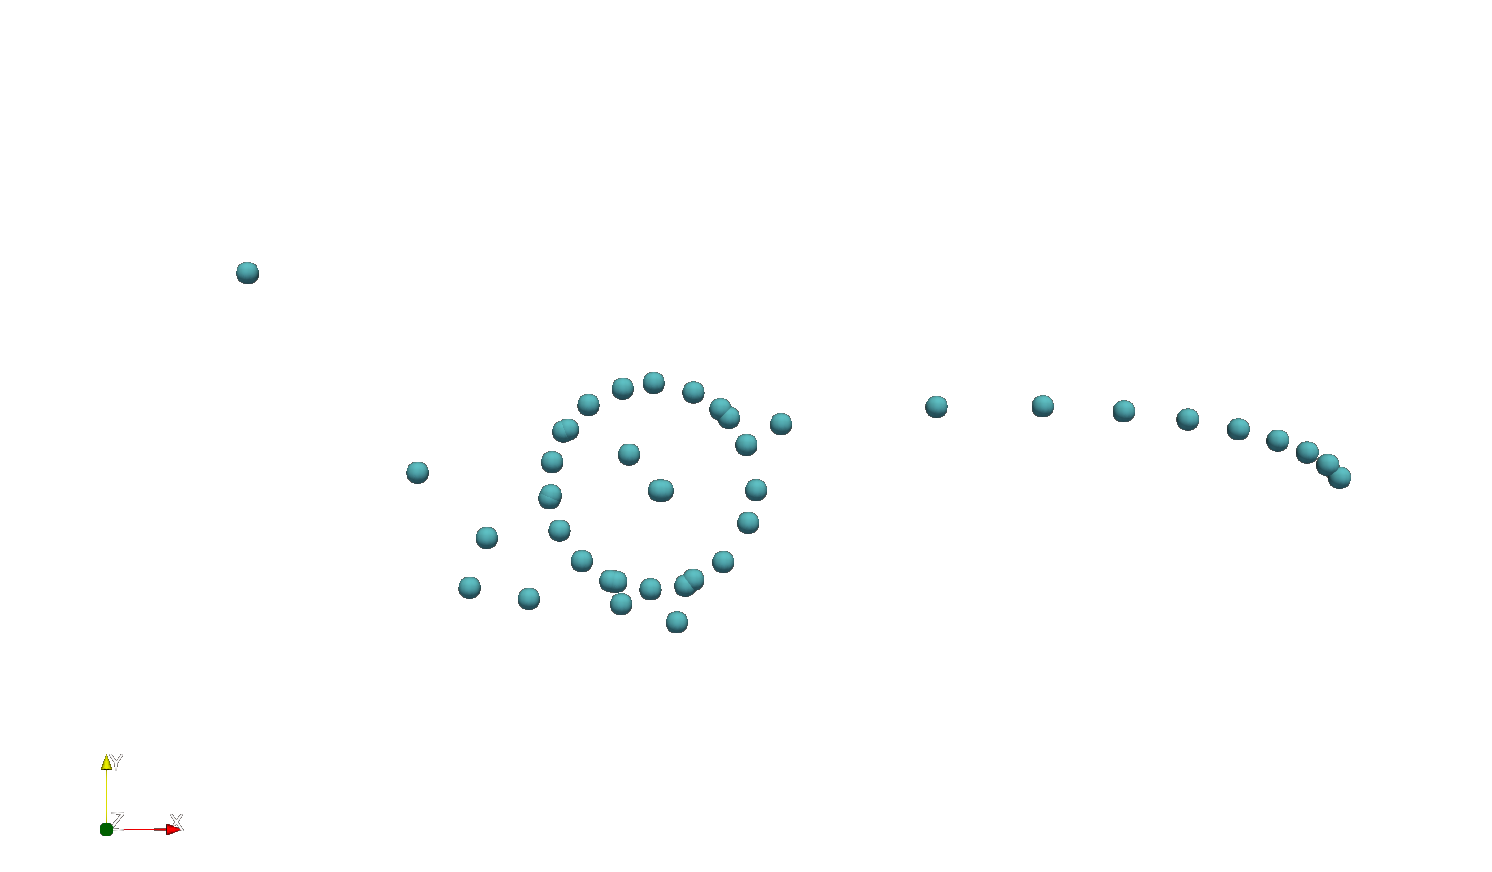
\includegraphics[width=0.9\textwidth]{media/t500_d2.24.png}
        \end{column}
    \end{columns}

    \vspace{0.5cm}
    Conclusion: \red{Results deviate for different $\Delta t$!}

    Follow-up question: \blue{How to choose an appropriate $\Delta t$?}
\end{frame}

\simpleframe\begin{frame}[fragile]{Code Refactoring done right}
    \begin{columns}
        \begin{column}{0.5\textwidth}
            \begin{lstlisting}
const std::array<double, 3>& x;
const std::array<double, 3>& v;
x = add_arrays(x, v);
            \end{lstlisting}
        \end{column}
        \begin{column}{0.5\textwidth}
            \begin{lstlisting}
const Vec3D& position;
const Vec3D& velocity;
position += velocity;
            \end{lstlisting}
        \end{column}
    \end{columns}

    \vspace{-0.25cm}
    We replaced \texttt{std::array<double, 3>} with a custom \texttt{Vec3} class that overloads operators for better readability.
    \vspace{0.25cm}

    \begin{lstlisting}
struct Vec3 {
    double x, y, z;

    Vec3& operator+=(const Vec3& other) {
        x += other.x;
        y += other.y;
        z += other.z;
        return *this;
    }
};
    \end{lstlisting}
\end{frame}

\simpleframe\begin{frame}[fragile]{Code Refactoring done right}{Fixing Particle Copying Issues}
    \begin{figure}
        \centering
        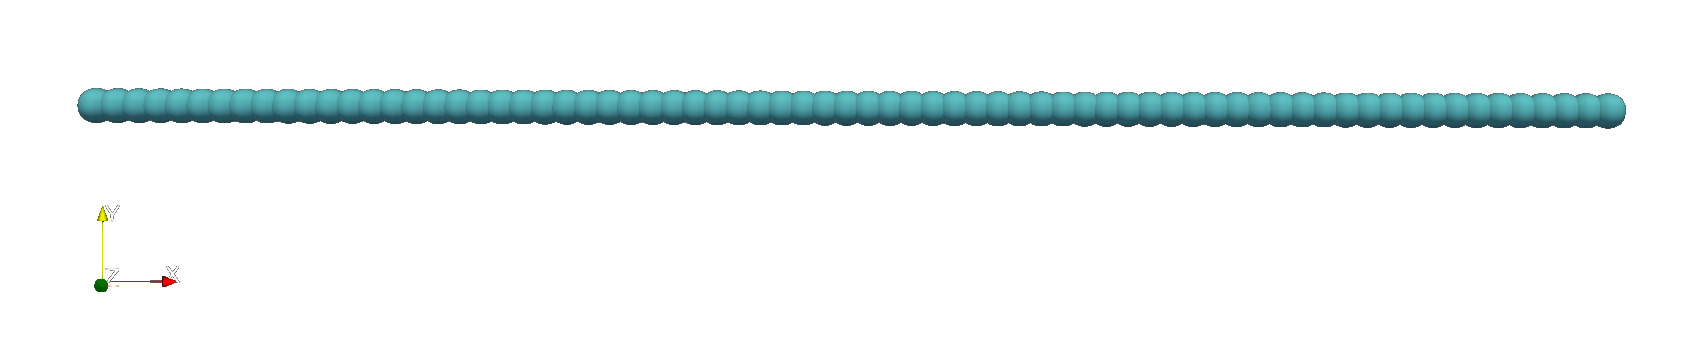
\includegraphics[width=0.6\textwidth]{media/simulation-line.png}
        \caption{One Particle Simulation}
    \end{figure}

    \vspace{-0.5cm}
    \begin{columns}
        \begin{column}{0.5\textwidth}
            \begin{lstlisting}
Iteration 9 finished.
Particle generated by copy!
Particle destructed!
Iteration 10 finished.
            \end{lstlisting}
        \end{column}
        \begin{column}{0.5\textwidth}
            \begin{lstlisting}
Iteration 8 finished.
Iteration 9 finished.
Iteration 10 finished.
Iteration 11 finished.
            \end{lstlisting}
        \end{column}
    \end{columns}
    \vspace{-0.75cm}
    \begin{columns}
        \begin{column}{0.5\textwidth}
% void add(const Particle p);
            \begin{lstlisting}
void VTKWriter::plot(ParticleContainer particles);
            \end{lstlisting}
        \end{column}
        \begin{column}{0.5\textwidth}
% void add(const Particle& p);
            \begin{lstlisting}
void VTKWriter::plot(ParticleContainer& particles);
            \end{lstlisting}
        \end{column}
    \end{columns}
\end{frame}

% \simpleframe\begin{frame}[fragile]{Code Refactoring done right}{Fixing Particle Copying Issues}
%     \blue{Our Fix:} The problem lay in \alert{missing \& in function signatures, causing unnecessary copies of Particle objects.}
% \end{frame}

\headerframe\begin{frame}{That's it – for now, at least}{Shaw! We thank you for your attention!}
    \begin{center}
        \begin{figure}
        \centering
        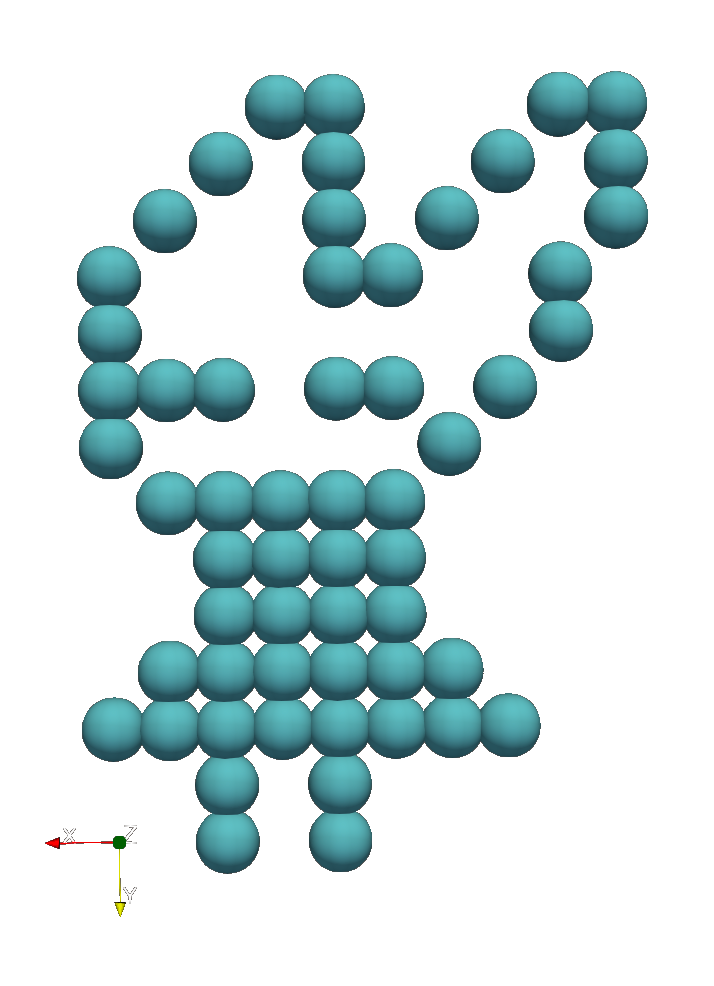
\includegraphics[width=0.35\textwidth]{media/shaw.png}
    \end{figure}
    \end{center}
\end{frame}

\end{document}
